%%%%%%%%%%%%%%%%%%%%%%%%%%%%%%%%%%%%%%%%%%%%%%%%%%%%%%%%%%%%%%%%%%%%%%%%%%%%%%%%
\chapter{РАЗРАБОТКА МОДУЛЯ АВТОМАТИЧЕСКОГО ИЗВЛЕЧЕНИЯ КОНТРАКТОВ ДЛЯ СИСТЕМЫ СТАТИЧЕСКОГО АНАЛИЗА BOREALIS}
\label{chapter:developing}
%%%%%%%%%%%%%%%%%%%%%%%%%%%%%%%%%%%%%%%%%%%%%%%%%%%%%%%%%%%%%%%%%%%%%%%%%%%%%%%%
В данном разделе описываются основные этапы разработки модуля автоматического извлечения контрактов для системы Borealis, который реализует описанную ранее технологию.

%%%%%%%%%%%%%%%%%%%%%%%%%%%%%%%%%%%%%%%%%%%%%%%%%%%%%%%%%%%%%%%%%%%%%%%%%%%%%%%%
\section{Архитектура прототипа}
%%%%%%%%%%%%%%%%%%%%%%%%%%%%%%%%%%%%%%%%%%%%%%%%%%%%%%%%%%%%%%%%%%%%%%%%%%%%%%%%
Под прототипом понимается программный модуль, реализующий предложенную методику автоматического извлечения контрактов. Процесс разработки можно разделить на две части: разработка модуля для системы Borealis и разработка библиотеки для работы со встраиваемой базой данных LevelDB\cite{leveldb}.

Структура каталогов модуля для системы Borealis приведена ниже (см. рисунок \ref{image:borealisStructure}).
\begin{figure}[h!]
\center{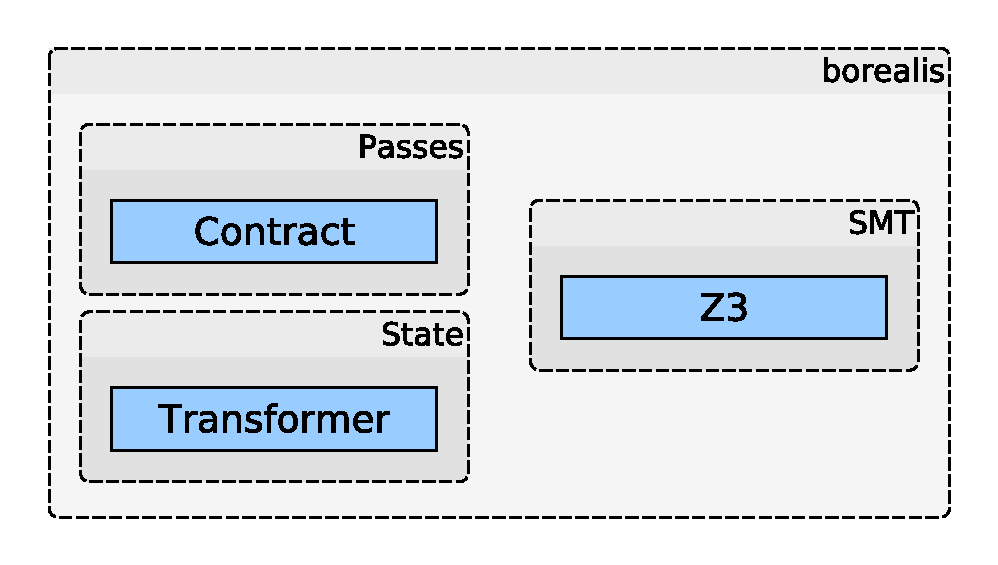
\includegraphics[width=0.75\linewidth]{borealisStructure}}
\caption{Структура каталогов модуля для системы Borealis}
\label{image:borealisStructure}
\end{figure}

Данный модуль реализует предложенную ранее технологию автоматического извлечения контрактов. То есть, он реализует следующие функции: анализ исходного кода и извлечение предварительного множества предикатов, работа с БД для записи/чтения результатов анализа, формирование контрактов для функции и добавление обнаруженных контрактов в систему для выполнения статического анализа.

Структура каталогов библиотеки для работы с LevelDB приведена ниже (см. рисунок \ref{image:leveldbStructure}).
\begin{figure}[h!]
\center{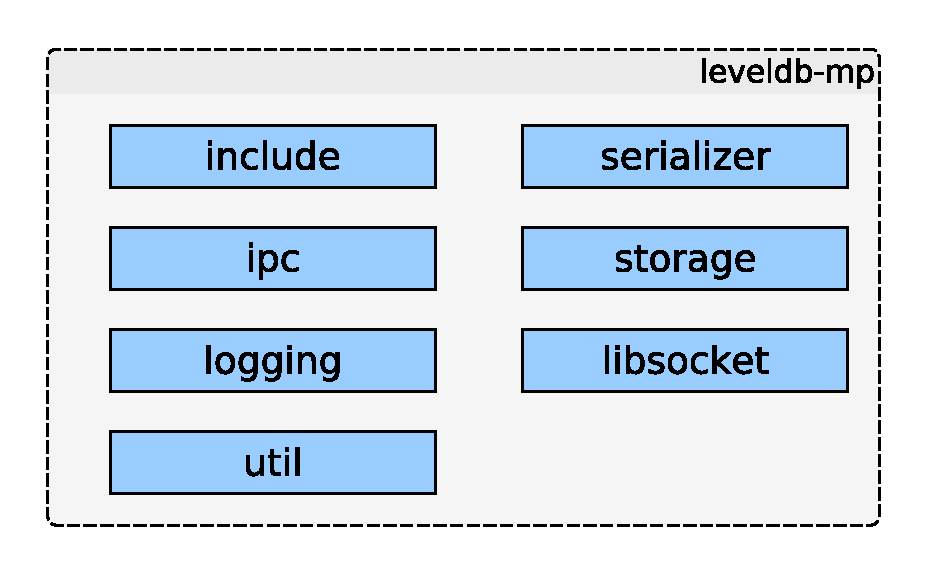
\includegraphics[width=0.75\linewidth]{leveldbStructure}}
\caption{Структура каталогов библиотеки для работы с LevelDB}
\label{image:leveldbStructure}
\end{figure}

В данном проекте реализуются два подпроекта: сервер для непосредственной работы с БД и клиент для подключения к этому серверу. БД используется для хранения результатов анализа.

Рассмотрим реализацию прототипа более подробно.